\chapter{Probabilités}

Ce chapitre aborde l'étude des probabilités sous l'angle du conditionnement, de la répétition d'épreuves indépendantes (la loi binomiale) et des théorèmes limites fondamentaux (inégalités de concentration et loi des grands nombres).

\section{Conditionnement et Indépendance}

\subsection{Probabilité conditionnelle}

\begin{definition}[Probabilité conditionnelle]
Soient $A$ et $B$ deux événements d'un univers $\Omega$, avec $P(A) \ne 0$.
La **probabilité conditionnelle de $B$ sachant $A$**, notée $P_A(B)$ (ou $P(B|A)$), est définie par :
\[
P_A(B) = \frac{P(A \cap B)}{P(A)}
\]
On en déduit la relation de probabilité de l'intersection : $P(A \cap B) = P(A) \times P_A(B)$.
\end{definition}

\subsection{Arbre pondéré et probabilités totales}

Pour modéliser une expérience à étapes, on utilise un **arbre pondéré** :

\begin{center}
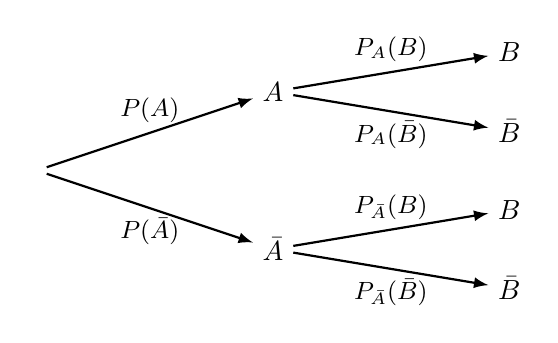
\begin{tikzpicture}[
  grow=right,
  level 1/.style={sibling distance=2cm, level distance=3cm},
  level 2/.style={sibling distance=1cm, level distance=3cm},
  edge from parent/.style={draw, ->, >=latex, thick},
  every node/.style={font=\sffamily}
]
  \node {}
    child {
      node {$\bar{A}$}
      child {
        node {$\bar{B}$}
        edge from parent node[below] {\small $P_{\bar{A}}(\bar{B})$}
      }
      child {
        node {$B$}
        edge from parent node[above] {\small $P_{\bar{A}}(B)$}
      }
      edge from parent node[below] {\small $P(\bar{A})$}
    }
    child {
      node {$A$}
      child {
        node {$\bar{B}$}
        edge from parent node[below] {\small $P_A(\bar{B})$}
      }
      child {
        node {$B$}
        edge from parent node[above] {\small $P_A(B)$}
      }
      edge from parent node[above] {\small $P(A)$}
    };
\end{tikzpicture}
\end{center}

Règles de calcul dans un arbre pondéré :
\begin{itemize}
    \item La somme des probabilités des branches issues d'un même nœud est égale à 1 (e.g. $P(A) + P(\bar{A}) = 1$ et $P_A(B) + P_A(\bar{B}) = 1$).
    \item La probabilité d'un chemin est le produit des probabilités des branches qui le composent (e.g. $P(A \cap B) = P(A) \times P_A(B)$).
\end{itemize}

\begin{theoreme}[Formule des probabilités totales]
Soit $A_1, A_2, \dots, A_n$ une partition de l'univers $\Omega$ (événements disjoints deux à deux et dont la réunion est $\Omega$). Pour tout événement $B$, on a :
\[
P(B) = P(A_1 \cap B) + P(A_2 \cap B) + \dots + P(A_n \cap B)
\]
C'est-à-dire, si les probabilités conditionnelles sont définies :
\[
P(B) = \sum_{i=1}^n P(A_i) \times P_{A_i}(B)
\]
\end{theoreme}

\subsection{Indépendance}

\begin{definition}[Événements indépendants]
Deux événements $A$ et $B$ sont **indépendants** si et seulement si :
\[
P(A \cap B) = P(A) \times P(B)
\]
Si $P(A) \ne 0$, cela équivaut à $P_A(B) = P(B)$.
\end{definition}

\section{Succession d'Épreuves Indépendantes et Loi Binomiale}

\subsection{Épreuve et schéma de Bernoulli}

\begin{definition}[Épreuve de Bernoulli]
Une **épreuve de Bernoulli** est une expérience aléatoire n'admettant que deux issues :
\begin{itemize}
    \item Le **succès**, noté $S$, de probabilité $p$ ($0 < p < 1$).
    \item L'**échec**, noté $\bar{S}$, de probabilité $q = 1-p$.
\end{itemize}
La variable aléatoire $X$ qui associe 1 au succès et 0 à l'échec suit la loi de Bernoulli de paramètre $p$.
\end{definition}

\begin{definition}[Schéma de Bernoulli]
Un **schéma de Bernoulli** est la répétition de $n$ épreuves de Bernoulli identiques et indépendantes.
\end{definition}

\subsection{Loi Binomiale}

Soit $X$ la variable aléatoire qui compte le nombre de succès à l'issue d'un schéma de Bernoulli de paramètres $n$ et $p$.

\begin{theoreme}[Loi Binomiale]
La variable aléatoire $X$ suit la **loi binomiale** de paramètres $n$ et $p$, notée $\mathcal{B}(n, p)$.
L'ensemble des valeurs prises par $X$ est $\llbracket 0, n \rrbracket$.
Pour tout entier $k \in \llbracket 0, n \rrbracket$, la probabilité d'obtenir exactement $k$ succès est :
\[
P(X = k) = \binom{n}{k} p^k (1-p)^{n-k}
\]
\end{theoreme}

\begin{propriete}[Indicateurs de la loi binomiale]
Si $X \sim \mathcal{B}(n, p)$, alors :
\begin{itemize}
    \item **Espérance** : $E(X) = np$
    \item **Variance** : $V(X) = np(1-p)$
    \item **Écart-type** : $\sigma(X) = \sqrt{np(1-p)}$
\end{itemize}
\end{propriete}

\section{Méthodes Clés}

\begin{methode}[Calculer des probabilités avec la loi binomiale]
Si une variable aléatoire $X$ suit la loi $\mathcal{B}(n, p)$ :
\begin{itemize}
    \item Pour calculer $P(X = k)$, on applique directement la formule : $\binom{n}{k} p^k (1-p)^{n-k}$.
    \item Pour calculer la probabilité d'avoir **au moins un succès** ($P(X \ge 1)$), on passe par l'événement contraire :
    \[
    P(X \ge 1) = 1 - P(X = 0) = 1 - (1-p)^n
    \]
\end{itemize}
\end{methode}

\begin{exemple}[Calcul binomial]
Un joueur lance un dé équilibré à 6 faces 5 fois de suite. On s'intéresse à l'obtention de la face « 6 ».
\begin{itemize}
    \item Chaque lancer est une épreuve de Bernoulli avec pour succès $S$ : « obtenir un 6 » ($p = 1/6$) et échec $\bar{S}$ ($q = 5/6$).
    \item Les lancers sont identiques et indépendants, donc la variable aléatoire $X$ comptant le nombre de « 6 » suit la loi binomiale $\mathcal{B}(5, 1/6)$.
    \item La probabilité d'obtenir exactement deux « 6 » est :
    \[
    P(X = 2) = \binom{5}{2} \left(\frac{1}{6}\right)^2 \left(\frac{5}{6}\right)^3 = 10 \times \frac{1}{36} \times \frac{125}{216} = \frac{1250}{7776} \approx 0,161
    \]
\end{itemize}
\end{exemple}

\section{Exercices d'Entraînement Résolus}

\subsection*{Exercice 1 : Conditionnement simple et arbre pondéré}
Dans une usine, deux machines A et B fabriquent des pièces électroniques. La machine A produit $60\%$ des pièces et la machine B produit $40\%$. Le taux de pièces défectueuses est de $2\%$ pour la machine A et de $3\%$ pour la machine B. On tire une pièce au hasard dans la production.
\begin{enumerate}
    \item Représenter la situation par un arbre pondéré.
    \item Calculer la probabilité que la pièce provienne de la machine A et soit défectueuse.
    \item Calculer la probabilité que la pièce soit défectueuse.
\end{enumerate}

\textbf{Solution :}
Soient les événements :
- $A$ : « la pièce est fabriquée par la machine A »
- $B$ : « la pièce est fabriquée par la machine B »
- $D$ : « la pièce est défectueuse »

\begin{enumerate}
    \item L'arbre pondéré représentant la situation est le suivant :
    \begin{center}
    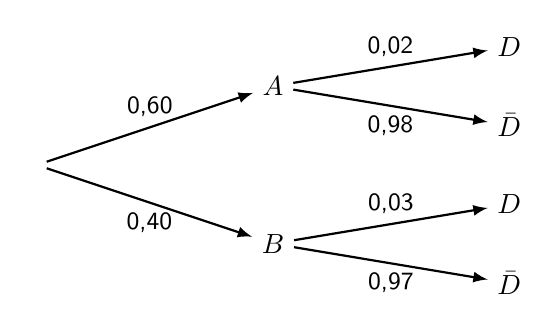
\begin{tikzpicture}[
      grow=right,
      level 1/.style={sibling distance=2cm, level distance=3cm},
      level 2/.style={sibling distance=1cm, level distance=3cm},
      edge from parent/.style={draw, ->, >=latex, thick},
      every node/.style={font=\sffamily}
    ]
      \node {}
        child {
          node {$B$}
          child {
            node {$\bar{D}$}
            edge from parent node[below] {\small 0,97}
          }
          child {
            node {$D$}
            edge from parent node[above] {\small 0,03}
          }
          edge from parent node[below] {\small 0,40}
        }
        child {
          node {$A$}
          child {
            node {$\bar{D}$}
            edge from parent node[below] {\small 0,98}
          }
          child {
            node {$D$}
            edge from parent node[above] {\small 0,02}
          }
          edge from parent node[above] {\small 0,60}
        };
    \end{tikzpicture}
    \end{center}
    
    \item On cherche à calculer la probabilité de l'intersection $A \cap D$ :
    \[
    P(A \cap D) = P(A) \times P_A(D) = 0,60 \times 0,02 = 0,012
    \]
    La probabilité que la pièce provienne de la machine A et soit défectueuse est de 0,012.
    
    \item D'après la formule des probabilités totales, comme $A$ et $B$ forment une partition de l'univers, on a :
    \[
    \begin{aligned}
    P(D) &= P(A \cap D) + P(B \cap D) \\
    &= P(A) \times P_A(D) + P(B) \times P_B(D) \\
    &= 0,60 \times 0,02 + 0,40 \times 0,03 \\
    &= 0,012 + 0,012 = 0,024
    \end{aligned}
    \]
    La probabilité que la pièce soit défectueuse est de 0,024 (soit $2,4\%$).
\end{enumerate}

\subsection*{Exercice 2 : Inversion des probabilités conditionnelles (Formule de Bayes)}
Avec les données de l'exercice 1, sachant que la pièce tirée au hasard est défectueuse, quelle est la probabilité qu'elle ait été fabriquée par la machine A ?

\textbf{Solution :}
On cherche à calculer la probabilité conditionnelle $P_D(A)$. Par définition :
\[
P_D(A) = \frac{P(A \cap D)}{P(D)}
\]
D'après les calculs de l'exercice 1, on a $P(A \cap D) = 0,012$ et $P(D) = 0,024$.
Calculons :
\[
P_D(A) = \frac{0,012}{0,024} = 0,5
\]
Sachant que la pièce est défectueuse, il y a exactement $50\%$ de chances qu'elle provienne de la machine A.

\subsection*{Exercice 3 : Indépendance d'événements}
On lance un dé équilibré à 6 faces. On note les événements suivants :
- $A$ : « obtenir un nombre pair »
- $B$ : « obtenir un multiple de 3 »
Les événements $A$ et $B$ sont-ils indépendants ?

\textbf{Solution :}
L'univers des possibles est $\Omega = \{1, 2, 3, 4, 5, 6\}$, muni de l'équiprobabilité.
Déterminons la composition et la probabilité des événements :
- $A = \{2, 4, 6\} \implies P(A) = \frac{3}{6} = \frac{1}{2}$.
- $B = \{3, 6\} \implies P(B) = \frac{2}{6} = \frac{1}{3}$.
L'événement $A \cap B$ correspond à « obtenir un nombre pair et multiple de 3 », c'est-à-dire :
- $A \cap B = \{6\} \implies P(A \cap B) = \frac{1}{6}$.
Comparons $P(A \cap B)$ et le produit $P(A) \times P(B)$ :
\[
P(A) \times P(B) = \frac{1}{2} \times \frac{1}{3} = \frac{1}{6}
\]
Puisque $P(A \cap B) = P(A) \times P(B)$, les événements $A$ et $B$ sont indépendants.

\subsection*{Exercice 4 : Loi binomiale - calculs de probabilités}
Une urne contient 3 boules blanches et 7 boules noires indiscernables au toucher. On effectue 4 tirages successifs d'une boule avec remise. Soit $X$ la variable aléatoire représentant le nombre de boules blanches obtenues.
\begin{enumerate}
    \item Préciser la loi suivie par la variable aléatoire $X$ et donner ses paramètres.
    \item Calculer la probabilité d'obtenir exactement 2 boules blanches.
    \item Calculer la probabilité d'obtenir au moins une boule blanche.
\end{enumerate}

\textbf{Solution :}
\begin{enumerate}
    \item Chaque tirage est une épreuve de Bernoulli dont le succès est « obtenir une boule blanche », de probabilité $p = \frac{3}{10} = 0,3$, et l'échec est de probabilité $1-p = 0,7$.
    Puisque les tirages sont effectués avec remise, ils sont identiques et indépendants. La variable aléatoire $X$ comptant le nombre de succès sur 4 répétitions suit donc la loi binomiale de paramètres $n = 4$ et $p = 0,3$, notée $\mathcal{B}(4; 0,3)$.
    
    \item On cherche à calculer $P(X = 2)$ :
    \[
    P(X = 2) = \binom{4}{2} p^2 (1-p)^{4-2} = 6 \times (0,3)^2 \times (0,7)^2 = 6 \times 0,09 \times 0,49 = 0,2646
    \]
    La probabilité d'obtenir exactement 2 boules blanches est de 0,2646.
    
    \item On cherche à calculer $P(X \ge 1)$. Utilisons l'événement contraire, qui est $\{X = 0\}$ :
    \[
    P(X \ge 1) = 1 - P(X = 0) = 1 - \binom{4}{0} (0,3)^0 (0,7)^4 = 1 - 1 \times 1 \times 0,2401 = 0,7599
    \]
    La probabilité d'obtenir au moins une boule blanche est de 0,7599.
\end{enumerate}

\subsection*{Exercice 5 : Indicateurs de la loi binomiale}
Un candidat répond complètement au hasard aux 20 questions d'un questionnaire à choix multiples (QCM). Pour chaque question, 4 réponses sont proposées, une seule étant correcte.
Soit $X$ la variable aléatoire égale au nombre de réponses correctes obtenues par le candidat.
\begin{enumerate}
    \item Déterminer la loi de probabilité de $X$.
    \item Calculer l'espérance mathématique $E(X)$ et interpréter ce résultat.
    \item Calculer la variance $V(X)$ et l'écart-type $\sigma(X)$ (arrondi à $10^{-2}$).
\end{enumerate}

\textbf{Solution :}
\begin{enumerate}
    \item Le candidat répond au hasard de manière indépendante à 20 questions. Chaque question a une probabilité de succès égale à $p = 0,25$ (1 réponse correcte sur 4).
    La variable aléatoire $X$ suit donc la loi binomiale de paramètres $n = 20$ et $p = 0,25$, soit $\mathcal{B}(20; 0,25)$.
    
    \item L'espérance mathématique de la loi binomiale est donnée par $E(X) = n p$ :
    \[
    E(X) = 20 \times 0,25 = 5
    \]
    Interprétation : En répondant complètement au hasard, le candidat peut s'attendre à obtenir en moyenne 5 bonnes réponses sur les 20 questions.
    
    \item La variance est :
    \[
    V(X) = n p (1-p) = 20 \times 0,25 \times 0,75 = 3,75
    \]
    L'écart-type est :
    \[
    \sigma(X) = \sqrt{V(X)} = \sqrt{3,75} \approx 1,94
    \]
\end{enumerate}

\subsection*{Exercice 6 : Événements indépendants avec la loi binomiale}
Soit $X$ une variable aléatoire suivant la loi binomiale $\mathcal{B}(2, p)$ avec $p \in ]0, 1[$.
Les événements $A : \{X \ge 1\}$ et $B : \{X \le 1\}$ peuvent-ils être indépendants ?

\textbf{Solution :}
Les valeurs possibles pour $X$ sont 0, 1 et 2, avec les probabilités suivantes :
- $P(X=0) = (1-p)^2$
- $P(X=1) = 2p(1-p)$
- $P(X=2) = p^2$
Calculons les probabilités des événements :
- $P(A) = P(X \ge 1) = 1 - P(X = 0) = 1 - (1-p)^2 = 2p - p^2 = p(2-p)$
- $P(B) = P(X \le 1) = P(X = 0) + P(X = 1) = (1-p)^2 + 2p(1-p) = (1-p)(1-p+2p) = (1-p)(1+p) = 1 - p^2$
L'événement intersection est $A \cap B = \{X = 1\}$, d'où $P(A \cap B) = 2p(1-p)$.
Les événements $A$ et $B$ sont indépendants si et seulement si $P(A \cap B) = P(A) \times P(B)$ :
\[
2p(1-p) = p(2-p)(1-p^2) \iff 2p(1-p) = p(2-p)(1-p)(1+p)
\]
Puisque $p \in ]0, 1[$, on a $p \ne 0$ et $1-p \ne 0$. On peut simplifier l'égalité par $p(1-p)$ :
\[
2 = (2-p)(1+p) \iff 2 = 2 + 2p - p - p^2 \iff p - p^2 = 0 \iff p(1-p) = 0
\]
Or, comme $p \in ]0, 1[$, $p(1-p)$ n'est jamais nul. L'égalité est impossible.
Les événements $A$ et $B$ ne sont donc jamais indépendants, quelle que soit la valeur de $p \in ]0,1[$.

\section{Problèmes Résolus}

\subsection*{Problème 1 : Modélisation médicale (Faux positifs et Faux négatifs)}
Dans une population, une maladie touche $1\%$ des individus. On met au point un test de dépistage de cette maladie :
- Si un individu est malade, le test est positif dans $99\%$ des cas (sensibilité du test).
- Si un individu est sain, le test est négatif dans $95\%$ des cas (spécificité du test).
On choisit un individu au hasard. On note $M$ l'événement « l'individu est malade » et $T$ « le test est positif ».
\begin{enumerate}
    \item Modéliser la situation par un arbre pondéré.
    \item Calculer la probabilité que le test soit positif pour un individu choisi au hasard.
    \item Si le test d'un individu est positif, quelle est la probabilité qu'il soit réellement malade ? Commenter le résultat obtenu.
    \item Si le test est négatif, quelle est la probabilité que l'individu soit tout de même malade (cas d'un faux négatif) ?
\end{enumerate}

\textbf{Solution :}
\begin{enumerate}
    \item L'arbre pondéré traduisant la situation est :
    \begin{center}
    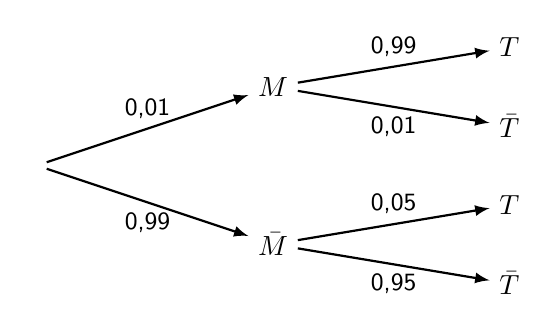
\begin{tikzpicture}[
      grow=right,
      level 1/.style={sibling distance=2cm, level distance=3cm},
      level 2/.style={sibling distance=1cm, level distance=3cm},
      edge from parent/.style={draw, ->, >=latex, thick},
      every node/.style={font=\sffamily}
    ]
      \node {}
        child {
          node {$\bar{M}$}
          child {
            node {$\bar{T}$}
            edge from parent node[below] {\small 0,95}
          }
          child {
            node {$T$}
            edge from parent node[above] {\small 0,05}
          }
          edge from parent node[below] {\small 0,99}
        }
        child {
          node {$M$}
          child {
            node {$\bar{T}$}
            edge from parent node[below] {\small 0,01}
          }
          child {
            node {$T$}
            edge from parent node[above] {\small 0,99}
          }
          edge from parent node[above] {\small 0,01}
        };
    \end{tikzpicture}
    \end{center}
    
    \item D'après la formule des probabilités totales, $\mathcal{P} = \{M, \bar{M}\}$ constituant une partition de l'univers :
    \[
    \begin{aligned}
    P(T) &= P(M \cap T) + P(\bar{M} \cap T) \\
    &= P(M) \times P_M(T) + P(\bar{M}) \times P_{\bar{M}}(T) \\
    &= 0,01 \times 0,99 + 0,99 \times 0,05 \\
    &= 0,0099 + 0,0495 = 0,0594
    \end{aligned}
    \]
    La probabilité que le test soit positif est de 0,0594 (soit $5,94\%$).
    
    \item On cherche à calculer la probabilité conditionnelle $P_T(M)$ :
    \[
    P_T(M) = \frac{P(M \cap T)}{P(T)} = \frac{0,0099}{0,0594} = \frac{99}{594} = \frac{1}{6} \approx 0,167
    \]
    Commentaire : Bien que le test soit individuellement très performant (99\% de sensibilité et 95\% de spécificité), un individu dont le test est positif n'a qu'environ $16,7\%$ de chances d'être réellement malade. Cela est dû au fait que la maladie est rare ($1\%$) : le nombre absolu de faux positifs ($4,95\%$) est bien plus important que le nombre de vrais positifs ($0,99\%$).
    
    \item On cherche à calculer la probabilité d'être malade sachant que le test est négatif, soit $P_{\bar{T}}(M)$ :
    \[
    P_{\bar{T}}(M) = \frac{P(M \cap \bar{T})}{P(\bar{T})} = \frac{P(M) \times P_M(\bar{T})}{1 - P(T)} = \frac{0,01 \times 0,01}{1 - 0,0594} = \frac{0,0001}{0,9406} \approx 0,000106
    \]
    La probabilité qu'un patient ayant un test négatif soit quand même malade est extrêmement faible (environ $0,01\%$).
\end{enumerate}

\subsection*{Problème 2 : Modélisation des parts de marché (Suites et Probabilités)}
Dans un pays, deux opérateurs de téléphonie mobile A et B se partagent le marché. On constate chaque année que :
- $15\%$ des clients de l'opérateur A changent pour B, tandis que $85\%$ lui restent fidèles.
- $20\%$ des clients de l'opérateur B changent pour A, tandis que $80\%$ lui restent fidèles.
Initialement (à l'année 0), l'opérateur A détient $70\%$ des clients et B en détient $30\%$.
Pour tout entier $n \ge 0$, on note $a_n$ la part de marché de A et $b_n$ la part de marché de B à l'année $n$.
\begin{enumerate}
    \item Justifier que pour tout entier $n \ge 0$, $a_n + b_n = 1$.
    \item Exprimer $a_{n+1}$ en fonction de $a_n$ et $b_n$, puis démontrer que :
    \[
    a_{n+1} = 0,65 a_n + 0,2
    \]
    \item Soit la suite $(u_n)$ définie pour tout entier $n \ge 0$ par $u_n = a_n - \frac{4}{7}$.
    Montrer que la suite $(u_n)$ est géométrique de raison $0,65$.
    \item Exprimer $u_n$ puis $a_n$ en fonction de $n$.
    \item Déterminer la limite de la suite $(a_n)$ lorsque $n \to +\infty$. Interpréter ce résultat.
\end{enumerate}

\textbf{Solution :}
\begin{enumerate}
    \item Les deux opérateurs A et B se partageant l'intégralité du marché sans perte de clients globale, la somme des proportions de clients de A et B est égale à la totalité du marché, soit $a_n + b_n = 1$ pour tout $n \ge 0$.
    
    \item À l'année $n+1$, les clients de A proviennent :
    - des clients fidèles de A de l'année précédente (proportion $0,85 a_n$).
    - des clients de B ayant migré chez A (proportion $0,20 b_n$).
    D'où :
    \[
    a_{n+1} = 0,85 a_n + 0,20 b_n
    \]
    Comme $b_n = 1 - a_n$, on obtient :
    \[
    a_{n+1} = 0,85 a_n + 0,20(1 - a_n) = 0,85 a_n + 0,2 - 0,2 a_n = 0,65 a_n + 0,2
    \]
    
    \item Exprimons $u_{n+1}$ en fonction de $u_n$ :
    \[
    \begin{aligned}
    u_{n+1} &= a_{n+1} - \frac{4}{7} \\
    &= (0,65 a_n + 0,2) - \frac{4}{7} \\
    &= 0,65 a_n + \frac{1}{5} - \frac{4}{7} \\
    &= 0,65 a_n + \frac{7 - 20}{35} \\
    &= 0,65 a_n - \frac{13}{35}
    \end{aligned}
    \]
    Factorisons par $0,65 = \frac{13}{20}$ :
    \[
    u_{n+1} = 0,65 \left( a_n - \frac{13/35}{13/20} \right) = 0,65 \left( a_n - \frac{13}{35} \times \frac{20}{13} \right) = 0,65 \left( a_n - \frac{20}{35} \right) = 0,65 \left( a_n - \frac{4}{7} \right) = 0,65 u_n
    \]
    La suite $(u_n)$ est donc géométrique de raison $q = 0,65$.
    
    \item Le premier terme de la suite est :
    \[
    u_0 = a_0 - \frac{4}{7} = 0,7 - \frac{4}{7} = \frac{7}{10} - \frac{4}{7} = \frac{49 - 40}{70} = \frac{9}{70}
    \]
    Par propriété des suites géométriques :
    \[
    u_n = u_0 \times q^n = \frac{9}{70} \times (0,65)^n
    \]
    On en déduit que :
    \[
    a_n = u_n + \frac{4}{7} = \frac{9}{70} \times (0,65)^n + \frac{4}{7}
    \]
    
    \item Comme $-1 < 0,65 < 1$, on a $\lim_{n \to +\infty} (0,65)^n = 0$.
    Par théorème d'opération sur les limites :
    \[
    \lim_{n \to +\infty} a_n = \frac{4}{7} \approx 0,571
    \]
    À long terme, la part de marché de l'opérateur A se stabilisera autour de $57,1\%$ et celle de l'opérateur B autour de $42,9\%$, indépendamment des parts de marché de départ.
\end{enumerate}

\subsection*{Problème 3 : Jeu de casino et espérance de gain}
Un joueur participe à un jeu dans un casino. Il lance un dé équilibré à 6 faces :
- S'il obtient un 6, il gagne 10 euros.
- S'il obtient 4 ou 5, il gagne 2 euros.
- S'il obtient 1, 2 ou 3, il perd 5 euros.
\begin{enumerate}
    \item Soit $X$ la variable aléatoire représentant le gain algébrique du joueur à l'issue d'une partie. Déterminer la loi de probabilité de $X$.
    \item Calculer l'espérance mathématique $E(X)$. Le jeu est-il favorable au joueur ?
    \item Le joueur effectue 5 parties successives et indépendantes. On note $Y$ le nombre de parties gagnantes (les parties où le joueur réalise un gain strictement positif).
    \begin{enumerate}
        \item Préciser la loi suivie par la variable aléatoire $Y$.
        \item Calculer la probabilité que le joueur gagne au moins 4 parties sur les 5 (arrondir à $10^{-4}$).
        \item Quelle est la probabilité que le joueur perde de l'argent sur l'ensemble des 5 parties dans le cas extrême où il ne gagne aucune partie ?
    \end{enumerate}
\end{enumerate}

\textbf{Solution :}
\begin{enumerate}
    \item Les valeurs possibles pour $X$ sont $10$, $2$ et $-5$. Les probabilités associées sont :
    - $P(X = 10) = P(\{6\}) = \frac{1}{6}$
    - $P(X = 2) = P(\{4, 5\}) = \frac{2}{6} = \frac{1}{3}$
    - $P(X = -5) = P(\{1, 2, 3\}) = \frac{3}{6} = \frac{1}{2}$
    La loi de probabilité de $X$ est donnée par le tableau :
    \begin{center}
    \begin{tabular}{|c|c|c|c|}
    \hline
    $x_i$ & $-5$ & $2$ & $10$ \\
    \hline
    $P(X = x_i)$ & $1/2$ & $1/3$ & $1/6$ \\
    \hline
    \end{tabular}
    \end{center}
    
    \item L'espérance mathématique est :
    \[
    E(X) = -5 \times \frac{1}{2} + 2 \times \frac{1}{3} + 10 \times \frac{1}{6} = -\frac{15}{6} + \frac{4}{6} + \frac{10}{6} = -\frac{1}{6} \approx -0,17 \text{ euro}
    \]
    Puisque $E(X) < 0$, le jeu est défavorable au joueur (il perd en moyenne environ 17 centimes d'euro par partie).
    
    \item Répétition de 5 épreuves de Bernoulli :
    \begin{enumerate}
        \item Une partie est gagnante si le gain est strictement positif, soit si $X \in \{2, 10\}$. La probabilité de succès pour une partie est :
        \[
        p = P(X = 2) + P(X = 10) = \frac{1}{3} + \frac{1}{6} = \frac{3}{6} = 0,5
        \]
        Comme les parties sont identiques et indépendantes, la variable aléatoire $Y$ suit la loi binomiale de paramètres $n = 5$ et $p = 0,5$, soit $\mathcal{B}(5; 0,5)$.
        
        \item On cherche $P(Y \ge 4)$ :
        \[
        \begin{aligned}
        P(Y \ge 4) &= P(Y = 4) + P(Y = 5) \\
        &= \binom{5}{4} (0,5)^4 (0,5)^1 + \binom{5}{5} (0,5)^5 (0,5)^0 \\
        &= 5 \times (0,5)^5 + 1 \times (0,5)^5 \\
        &= 6 \times 0,03125 = 0,1875
        \end{aligned}
        \]
        La probabilité que le joueur gagne au moins 4 parties est de 0,1875.
        
        \item Si le joueur ne gagne aucune partie ($Y=0$), cela signifie qu'il a perdu à chacune des 5 parties (il a obtenu 5 fois l'issue $-5$ euros). La probabilité de cet événement est :
        \[
        P(Y = 0) = \binom{5}{0} (0,5)^0 (0,5)^5 = 0,03125
        \]
        Dans ce cas, le gain total sur les 5 parties est $5 \times (-5) = -25$ euros.
    \end{enumerate}
\end{enumerate}
